Para el desarrollo de esta práctica, se desarrolló la topología siguiente en la cuál se conectaron 3 computadoras en total siendo la primera la que tenía implmentado el código de Python que fungía como cliente (figura \ref{image:top1}) y las otras dos que contenían los servidores configurados (figuras \ref{image:top2} y \ref{image:top3}).

\FloatBarrier
\begin{figure}[htbp!]
		\centering
			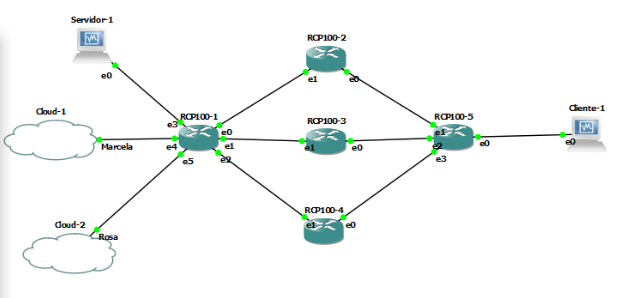
\includegraphics[width=.8 \textwidth]{images/top1}
		\caption{Computadora 1.}
		\label{image:top1}
\end{figure}
\FloatBarrier

En las figuras mostradas en la parte inferior se observa únicamente una cloud conectada con su propia computadora pues se realizó la conexión por medio de un túnel UDP.
\FloatBarrier
\begin{figure}[htbp!]
		\centering
			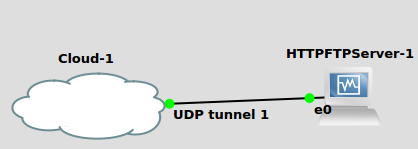
\includegraphics[width=.5 \textwidth]{images/top2}
		\caption{Computadora 2.}
		\label{image:top2}
\end{figure}
\FloatBarrier

\FloatBarrier
\begin{figure}[htbp!]
		\centering
			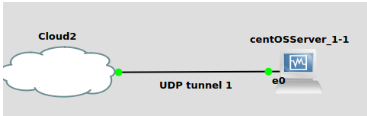
\includegraphics[width=.55 \textwidth]{images/top3}
		\caption{Computadora 3.}
		\label{image:top3}
\end{figure}
\FloatBarrier

La funcionalidad de esta topología constaba en comunicar el cliente desde donde se ejecutaron los sensores que monitorizaban el funcionamiento de cada uno de servidores almacenados en las computadoras 2 y 3.
\\ \par
La configuración de estos routers se realizaron por los 3 diferentes métodos que eran estático, RIP y OSPF. A continuación se muestran algunos de los comandos necesarios para la realización de dicha configuración en cada uno de los enrutadores.
\\ \par
\textbf{Enrutamiento estático}
\\ \par
La tabla de enrutamiento contiene la información más importante que usan los routers. Esta tabla
proporciona la información que usan los routers para reenviar los paquetes recibidos. Si la
información de la tabla de enrutamiento no es correcta, el tráfico se reenviará incorrectamente y posiblemente no llegue al destino. Para que se comprendan las rutas de tráfico, la resolución de
problemas y la manipulación del tráfico, es absolutamente necesario que se tengan conocimientos
sólidos sobre cómo leer y analizar una tabla de enrutamiento [1]. 
\FloatBarrier
\begin{figure}[htbp!]
		\centering
			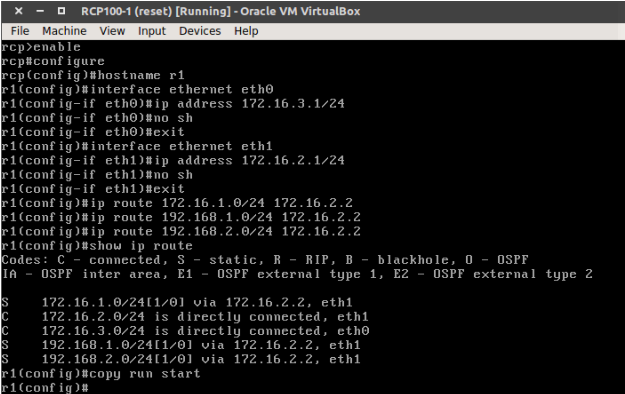
\includegraphics[width=.7 \textwidth]{images/estatico}
		\caption{Configuración enrutamiento estático.}
		\label{image:estatico}
\end{figure}
\FloatBarrier
\textbf{Enrutamiento RIP}
\\ \par
RIP es un protocolo dinámico y tiene 2 versiones (RIP y RIPv2). La versión 1 de RIP es con clase (no soporta VLSM), no utiliza autenticación y utiliza broadcast. La versión 2 de RIP es sin clase (soporta VLSM), añade la autenticacion y utiliza multicast.
La base de la configuración del protocolo RIP en Cisco se encuentra en el comando network  [2].
Dicho comando cumple con dos propósitos:
\begin{itemize}
\item Informar a RIP sobre qué interfaces intervienen en el envío y recepción de actualizaciones de enrutamiento.
\item Pedir a RIP que anuncie a los demás routers la existencia de la red.
\end{itemize}
\FloatBarrier
\begin{figure}[htbp!]
		\centering
			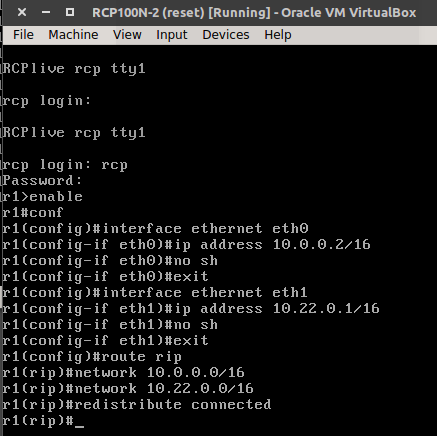
\includegraphics[width=.45 \textwidth]{images/rip}
		\caption{Configuración RIP.}
		\label{image:rip}
\end{figure}
\FloatBarrier


\textbf{Enrutamiento OSPF}
\\ \par
Open Shortest Path First (OSPF), camino más corto primero, es un protocolo de red para encaminamiento jerárquico de pasarela interior o Interior Gateway Protocol (IGP), que usa el algoritmo SmoothWall Dijkstra enlace-estado para calcular la ruta idónea entre dos nodos cualesquiera de un sistema autónomo.

Su medida de métrica se denomina cost, y tiene en cuenta diversos parámetros tales como el ancho de banda y la congestión de los enlaces. OSPF construye además una base de datos enlace-estado (Link-State Database, LSDB) idéntica en todos los routers de la zona.

Una red OSPF se puede descomponer en regiones (áreas) más pequeñas. Hay un área especial llamada área backbone que forma la parte central de la red a la que se encuentran conectadas el resto de áreas de la misma. Las rutas entre las diferentes áreas circulan siempre por el backbone, por lo tanto todas las áreas deben conectar con el backbone. Si no es posible hacer una conexión directa con el backbone, se puede hacer un enlace virtual entre redes [3].
\FloatBarrier
\begin{figure}[htbp!]
		\centering
			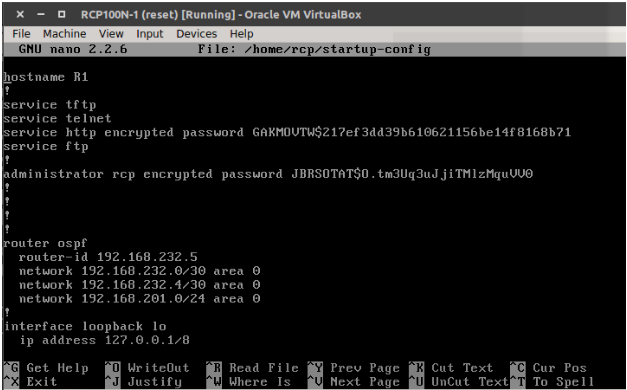
\includegraphics[width=.8 \textwidth]{images/ospf}
		\caption{Configuración OSPF.}
		\label{image:ospf}
\end{figure}
\FloatBarrier